\section{Conception}\label{sec:design}
La communication dans \acrshort{tor} se fait au travers de flux de données composés de cellules et empruntant des circuits prédéfinis.

\begin{enumerate}
    \item \ref{subsec:cellule} \nameref{subsec:cellule} de types contrôle ou relais, leurs fonctions sont spécifiques.
    \item \ref{subsec:circuit} \nameref{subsec:circuit} construits via des cellules de contrôles, ils transmettent les données via des cellules de relais.
\end{enumerate}
\subsection{Cellules}\label{subsec:cellule}

D'une taille fixe de 512 octets, elles se divisent en deux parties principales : un en-tête (header) et une charge utile (payload). 
L'en-tête contient un identifiant de circuit (circID) et une commande (CMD), comme illustré ci-dessous dans le schéma de la Figure \ref{fig:structure-cellule}.

\begin{figure}[h!]
    \centering
    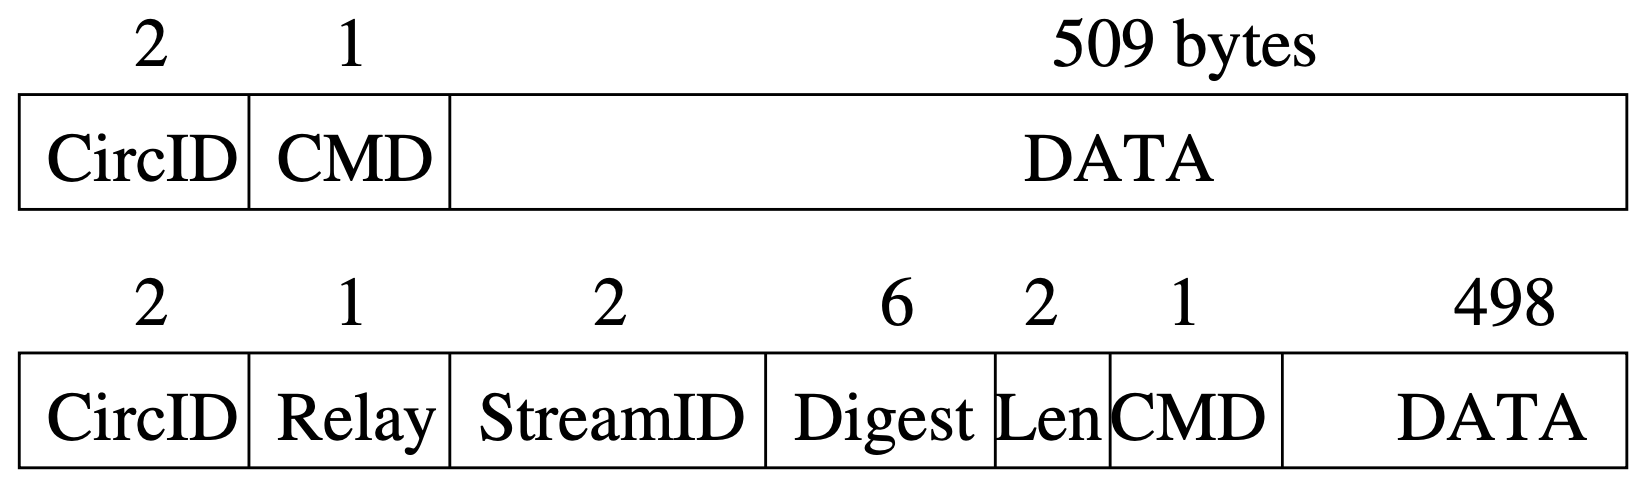
\includegraphics[width=0.5\linewidth]{Images/Diagrams/cellule.png}
    \caption{Structure de cellule vs structure d'une cellule de relais. \cite[Tor: The Second-Generation Onion Router]{dingledine_tor_2004}}
    \label{fig:structure-cellule}
\end{figure}

Il existe deux types de cellules distincts:
\begin{enumerate}
    \item Contrôle : les cellules de contôle sont traitées directement par le noeud qui les reçoit; leurs fonctions sont administratives: initialisation, maintenance et clôture du circuit.
    \item Relais : les cellules de relais permettent le transfert de bout en bout des données utilisateur, leurs fonctions concernent le flux de données
\end{enumerate}

Le tableau \ref{tab:cellules-tor} "\nameref{tab:cellules-tor}" ci-dessous reprend l'ensemble des différents types de cellules utilisées dans \acrshort{tor}.
Les commandes y sont spécifiques aux type dont il est question.

\begin{table}[htbp]
    \centering
    \begin{tabularx}{\textwidth}{
        >{\raggedright\arraybackslash}p{2cm} 
        >{\raggedright\arraybackslash}X 
        >{\raggedright\arraybackslash}X}
            \toprule
            \rowcolor[HTML]{EFEFEF}
            \textbf{Type}           & \textbf{Commandes}        & \textbf{Fonctions} \\
            \midrule
            Contrôle & PADDING & Garder la connexion active \\
            & CREATE & Établir un nouveau circuit \\
            & CREATED & Confirmer la création du circuit \\
            & DESTROY & Fermer un circuit \\
            \addlinespace
            Relais & RELAY\_BEGIN & démarrer une connexion \acrshort{tcp} \\
            & RELAY\_DATA & transfert de données \\
            & RELAY\_END & fermer une connexion \acrshort{tcp} \\
            & RELAY\_CONNECTED & confirmer l'établissement de la connexion \acrshort{tcp} \\
            & RELAY\_EXTEND & étendre un circuit à un autre nœud \\
            & RELAY\_TRUNCATED & signaler une coupure de circuit partielle \\
            & RELAY\_SENDME & contrôle de congestion (demande de données) \\
            \bottomrule
    \end{tabularx}
    \caption{Comparaison des Types de Cellules et de leurs commandes dans le Réseau Tor}
    \label{tab:cellules-tor}
\end{table}

\newpage
\subsection{Circuits}\label{subsec:circuit}

Contrairement à la première génération de routage onion, chaque circuit peut multiplexer différents flux TCP.
Ces circuits sont reconstruits chaque minute par les \acrshort{op} afin de limiter les liens entre flux (rotation périodique).

Les circuits sont composés de trois types de n\oe uds:
\begin{itemize}
    \item Gardien d'entrée
    \item Noeud(s) intermédiaire(s)
    \item Noeud de sortie
\end{itemize}


Sur la Figure \ref{fig:flowdiagram} "\nameref{fig:flowdiagram}" ci-dessous, "\acrshort{or} 1" représente le "Gardien d'entrée" tandis que "\acrshort{or} 2" représente le "Noeud de sortie".
Le processus est initié par l'expéditeur, qui utilise des cellules de contrôle afin de construire le circuit.
Lorsque la connection avec le premier  \acrshort{or}  est établie via une cellule de création, le processus continue jusqu'à atteindre la destination finale.
Une fois le circuit construit, des cellules de relais le parcourent jusqu'à atteindre la destination et retourner le résultat à l'expéditeur.

\begin{figure}[h!]
    \centering
    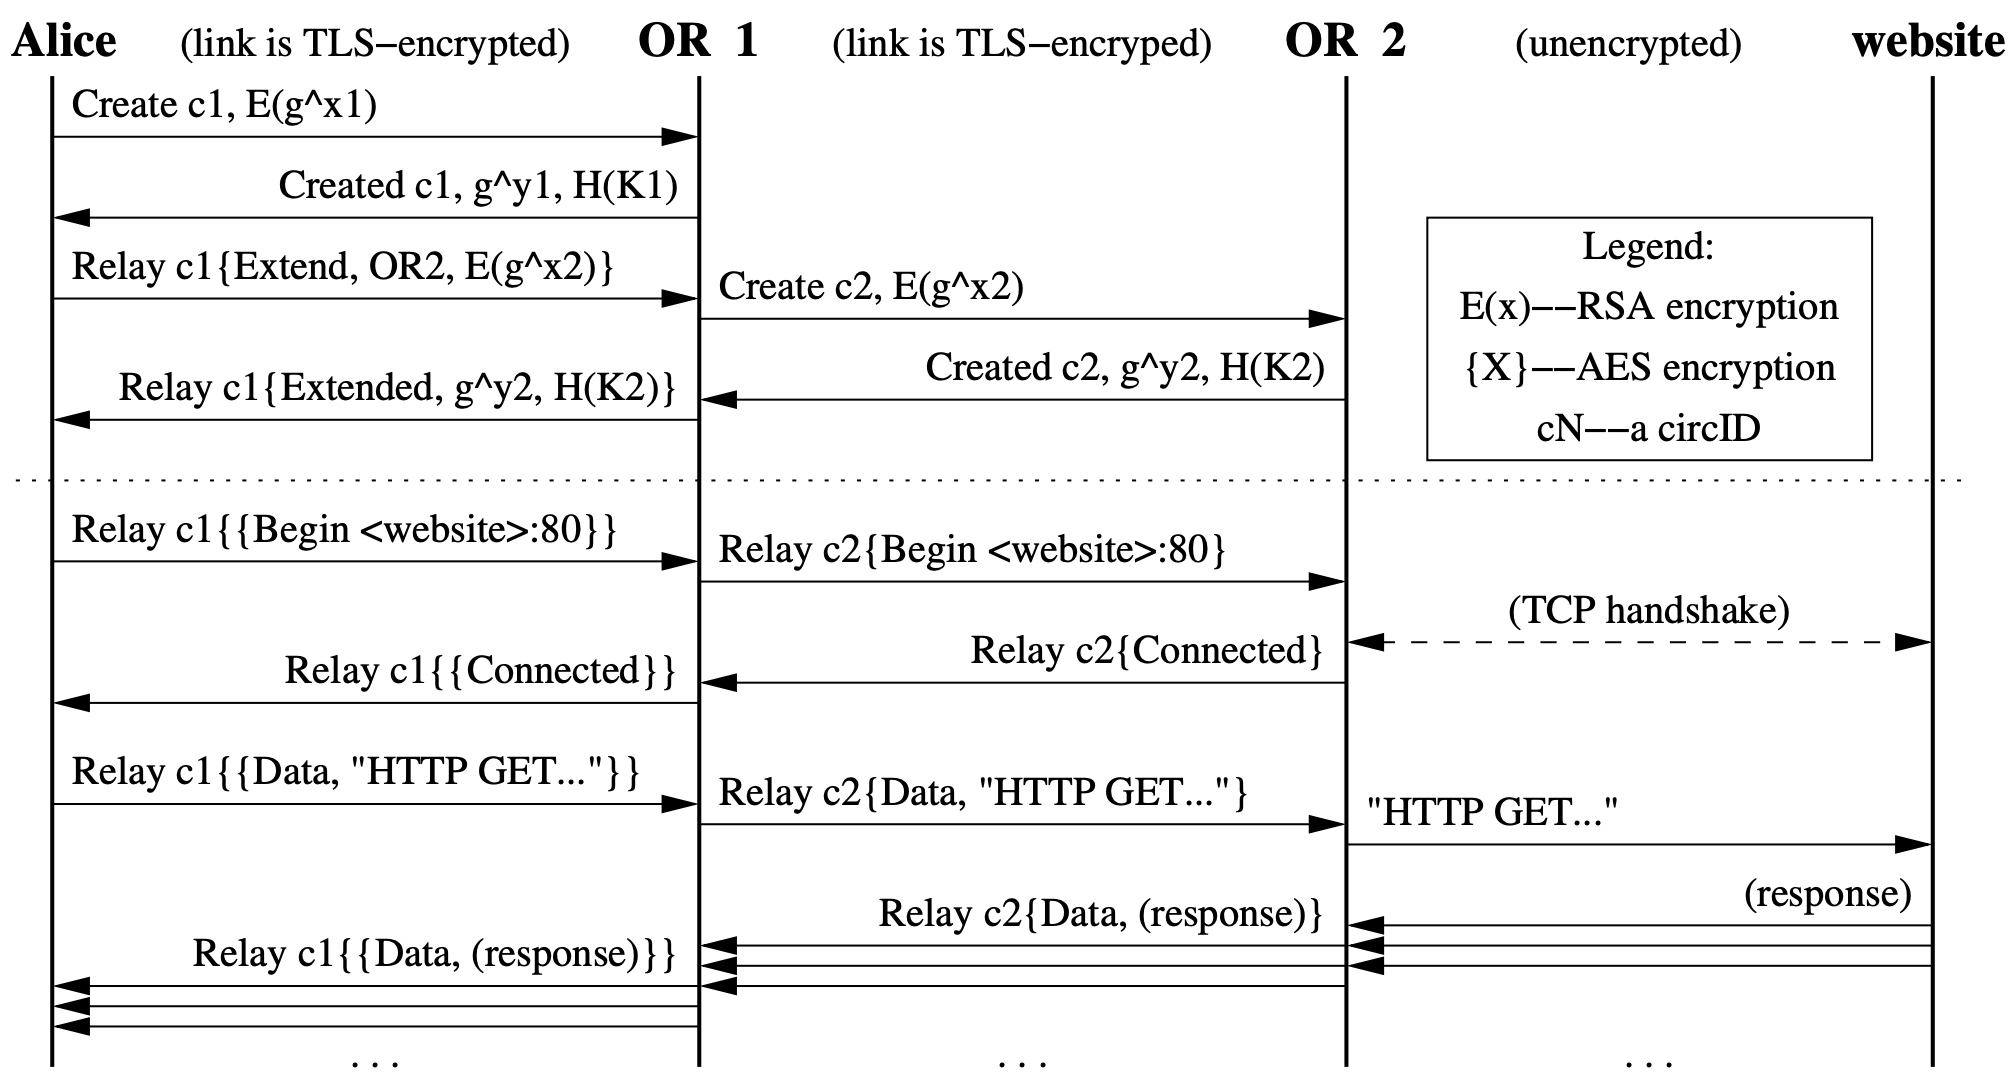
\includegraphics[width=\linewidth]{Images/Diagrams/flow.png}
    \caption{Circuit à deux Routeurs Onions permettant à Alice de joindre un site web.\cite[Tor: The Second-Generation Onion Router]{dingledine_tor_2004}}
    \label{fig:flowdiagram}
\end{figure}
